\documentclass[tikz]{standalone}
\begin{document}

% first method
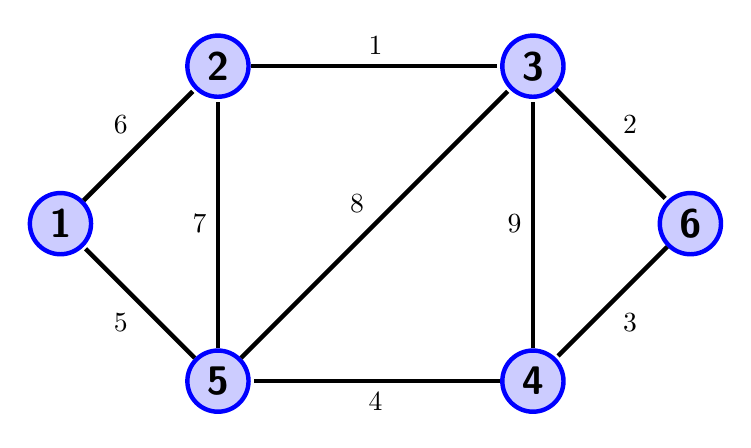
\begin{tikzpicture}[shorten >=1pt, auto, node distance=3cm, ultra thick,
   node_style/.style={circle,draw=blue,fill=blue!20!,font=\sffamily\Large\bfseries},
   edge_style/.style={draw=black, ultra thick}]

    \node[node_style] (v1) at (-2,2) {2};
    \node[node_style] (v2) at (2,2) {3};
    \node[node_style] (v3) at (4,0) {6};
    \node[node_style] (v4) at (2,-2) {4};
    \node[node_style] (v5) at (-2,-2) {5};
    \node[node_style] (v6) at (-4,0) {1};
    \draw[edge_style]  (v1) edge node{1} (v2);
    \draw[edge_style]  (v2) edge node{2} (v3);
    \draw[edge_style]  (v3) edge node{3} (v4);
    \draw[edge_style]  (v4) edge node{4} (v5);
    \draw[edge_style]  (v5) edge node{5} (v6);
    \draw[edge_style]  (v6) edge node{6} (v1);
    \draw[edge_style]  (v5) edge node{7} (v1);
    \draw[edge_style]  (v5) edge node{8} (v2);
    \draw[edge_style]  (v4) edge node{9} (v2);
    \end{tikzpicture}

% Second method
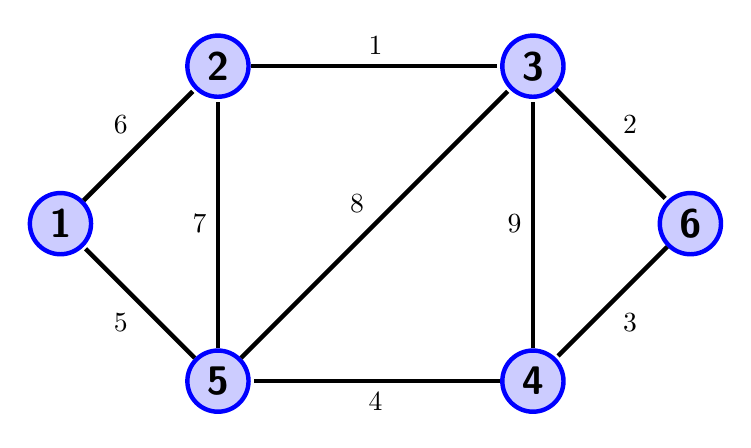
\begin{tikzpicture}[shorten >=1pt, auto, node distance=3cm, ultra thick]
   \begin{scope}[every node/.style={circle,draw=blue,fill=blue!20!,font=\sffamily\Large\bfseries}]
    \node (v1) at (-2,2) {2};
    \node (v2) at (2,2) {3};
    \node (v3) at (4,0) {6};
    \node (v4) at (2,-2) {4};
    \node (v5) at (-2,-2) {5};
    \node (v6) at (-4,0) {1};
   \end{scope}
   \begin{scope}[every edge/.style={draw=black,ultra thick}]
    \draw  (v1) edge node{1} (v2);
    \draw  (v2) edge node{2} (v3);
    \draw  (v3) edge node{3} (v4);
    \draw  (v4) edge node{4} (v5);
    \draw  (v5) edge node{5} (v6);
    \draw  (v6) edge node{6} (v1);
    \draw  (v5) edge node{7} (v1);
    \draw  (v5) edge node{8} (v2);
    \draw  (v4) edge node{9} (v2);
   \end{scope}
\end{tikzpicture}

% Third method    
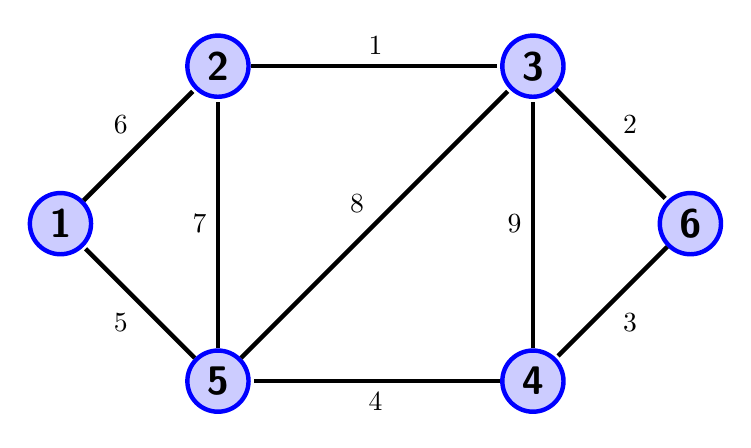
\begin{tikzpicture}[shorten >=1pt, auto, node distance=3cm, ultra thick,
   edge_style/.style={draw=black, ultra thick}]

   \foreach [count=\i] \x/\y/\t in {-2/2/2, 2/2/3, 4/0/6, 2/-2/4, -2/-2/5, -4/0/1}
     \node [circle,draw=blue,fill=blue!20!,font=\sffamily\Large\bfseries]
        (v\i) at (\x,\y) {\t};

   \foreach \i/\j/\t in {1/2/1, 2/3/2, 3/4/3, 4/5/4, 5/6/5, 6/1/6, 5/1/7, 5/2/8, 4/2/9}
    \draw [edge_style]  (v\i) edge node{\t} (v\j);
\end{tikzpicture}
\end{document}
